% !TEX root = ../Main.tex
When operating a fusion reactor a continous process of diagnostics is necessary in order to optimise the plasma for the fusion process. One of the active diagnostic methods are interferometry.
The goal here for this part of the paper is to measure the plasma electron density in the Danish Tokamak Undertaking reactor.
\subsection{Cutt-off and Source frequency}
Using a interferometer one can measure the electron density \(n_e\) of the plasma. The refractive index of electromagnetic waves depend on the electron density and plasma frequency \(\omega_p\) proportionally:
\begin{align}
	\omega_p^2 \propto n_e
\end{align}
For O-mode plasma waves the refractive index is:
\begin{align}
	N_{\mathrm{O}} = \sqrt{1-\frac{\omega_p^2}{\omega^2}}
\end{align}
with \(\omega\) being the probing wave frequency.
The plasma will reflect the beam if the plasma frequency is larger than the beam frequency so
\begin{align}
	\omega > \omega_p = \sqrt{n_e\frac{e^2}{\epsilon_0 m_{e0}}}
\end{align}
So for a given frequency, the plasma must not exceed a critical cut off electron density:
\begin{align}
	n_e < n_c      & = \omega^2\frac{\epsilon_0\cdot m_{e0}}{e^2} \label{nenc} \\
	               & \qq*{which gives} \nonumber                               \\
	N_{\mathrm{O}} & = \sqrt{1-\frac{n_e}{n_c}}\label{NO}
\end{align}
With a probing frequency much higher than the plasma frequency and the critical density much higher than the electron density \cref{NO} can be approximated by:
\begin{align}
	N_{\mathrm{O}} & = \sqrt{1-\frac{n_e}{n_c}} \approx 1-\frac{1}{2}\frac{n_e}{n_c} 0 1-\frac{\omega_p^2}{2\omega^2}
\end{align}
With sufficient accuracy, the linear dependence of the O-mode refractive index on the electron density is obtained if the normalised quantities obey:
\begin{align}
	\frac{n_e}{n_c} \leq 0.4 \quad \frac{\omega_p}{\omega} \leq 0.6
\end{align}
We must calculate the phase shift as one beam travels in vacuum by the length \(L_V\) and one wave travels in the plasma by the length \(L_P\). The phase shift in terms of \(2 \pi\) is equal to the optical difference divided by the wavelength. With the refractive index in vacuum, \(N_V=1\), this yields:
\begin{align}
	\frac{\Phi}{2\pi} & = \frac{\Delta L_{opt}}{\lambda} = \frac{\int_{x_1}^{x_2}\pqty{N_V-N_{\mathrm{O}}(x')}\dd{x'}}{\lambda} \approx \frac{1}{2\lambda n_c}\int_{0}^{x}n_e(x')\dd{x'} \nonumber \\
	                  & = 4.48\times 10^{-16} \pqty{\frac{\lambda}{\si{\meter}}}\int_{0}^{x}\pqty{\frac{n_e(x')}{\si{\per\meter\cubed}}}\pqty{\frac{\dd{x'}}{\si{\meter}}} \label{Phipi}
\end{align}
Assuming a Gaussian distribution, the electron density at \(\pm\infty\) is approximately equal to the densities just inside the reactor walls. Therefore
\begin{align}
	\int_{-\infty}^{\infty}n_e \exp\pqty{-\frac{(y-b)^2}{2c^2}}\dd{y} \approx n_e\ c\ \sqrt{2\pi}\label{c}
\end{align}
With the density at the centre given as:
\begin{align}
	\SI{e16}{\per\meter\cubed} \leq n_e \leq \SI{e18}{\per\meter\cubed},
\end{align}
The \(c\) in \cref{c} is the width of the Gaussian distribution and must fit inside the reactor. The DTU tokamak has a minor diameter of \SI{0.25}{\meter}. Thus
\begin{align}
	\frac{\Phi}{2\pi} \approx 4.48\times 10^{-16}\pqty{\frac{\lambda}{\si{\meter}}}n_e\SI{0.25}{\meter}\sqrt{2\pi} & = 1.12\times 10^{-16}\ n_e  \pqty{\frac{\sqrt{2\pi} c}{\omega\si{\meter}}} \nonumber \\
	                                                                                                               & = 8.416\times 10^{-8}\pqty{\frac{n_e}{\omega\si{\second}}}\label{Phipi2}
\end{align}
Remembering \cref{nenc}
\begin{align}
	\omega^2\frac{\epsilon_0\ m_{e0}}{e^2} & = \omega^2\frac{\SI{8.854e-12}{\farad\per\meter}\ \SI{9.109e-31}{\kilo\gram}}{\SI{1.602e-19}{\coulomb}} \\
	                                       & \Downarrow\nonumber                                                                                     \\
	n_e                                    & < 0.000314\omega^2 \label{co}
\end{align}
Where any units has been disregarded. We want the largest possible phase shift which means that the lower the frequency the better. However cutoff must first be taken into account.
Since the cutoff is given by \cref{co} and since we want to measure densities up to \SI{e18}{\per\meter\cubed} the minimum frequency of the wave is
\begin{align}
	\frac{\omega}{2\pi} & > \frac{\sqrt{\frac{\SI{e18}{\per\meter\cubed}}{0.000314}}}{2\pi} \\
	                    & \Downarrow\nonumber                                               \\
	f                   & \approx \SI{9}{\giga\hertz}
\end{align}
Given the available emitters, the best emitter is therefore the one with \(f=60\si{GHz}\).
\subsection{Beam Phaseshifts}
\begin{wrapfigure}[12]{r}{.5\textwidth}
	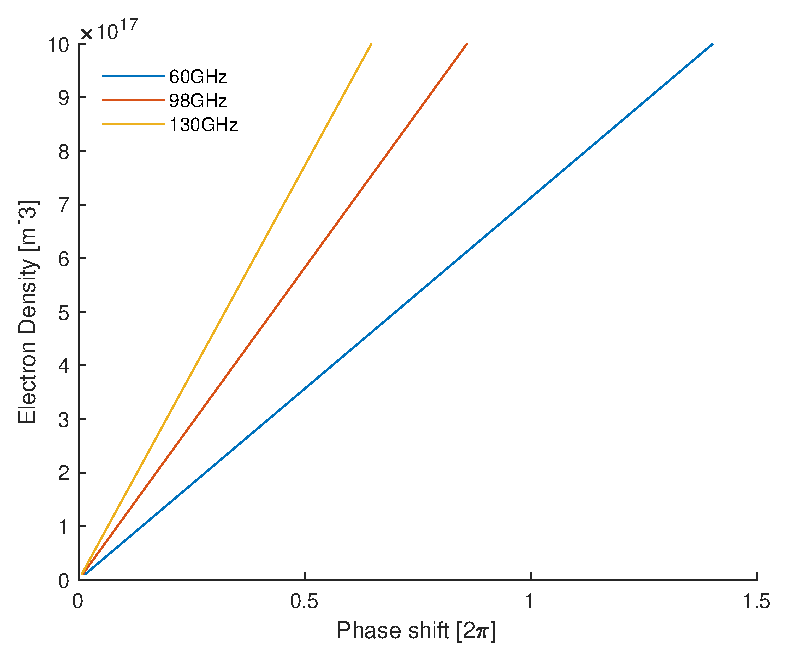
\includegraphics[width=.5\textwidth]{MatlabFigures/PhaseShift/PhaseShift.eps}
	\caption{Electron densities for different wavelengths and phaseshifts}
	\label{PhPlot}
\end{wrapfigure}
The goal of the interferometer is to find the phaseshift between the microwave beam in vacuum and in plasma. Our suggestion is a setup involving a interferometer emitting a beam through the center of the reactor. The first measurement would be through vacuum to find the source phase. Afterwards phase measurements can be conducted with an active plasma in the reactor.
So by first measuring the phase of the probing beam in vacuum, one can simply measure the phase shift.\\
We know from \cref{Phipi,c,,Phipi2} that:
\begin{align}
	\frac{\Phi}{2\pi} = 8.416\times 10^{-8}\pqty{\frac{n_e}{\omega\si{\second}}}
\end{align}
So for different average electron densities through the plasma, one can plot the resulting phaseshifts.
Using the code in \cref{PSD} the plot in \cref{PhPlot} is generated. The measured phase shift is then correlated to an electron density using \cref{PhPlot}.
\subsection{Evolving beam width}
\begin{wrapfigure}[14]{r}{.4\textwidth}
	\vspace{-5mm}
	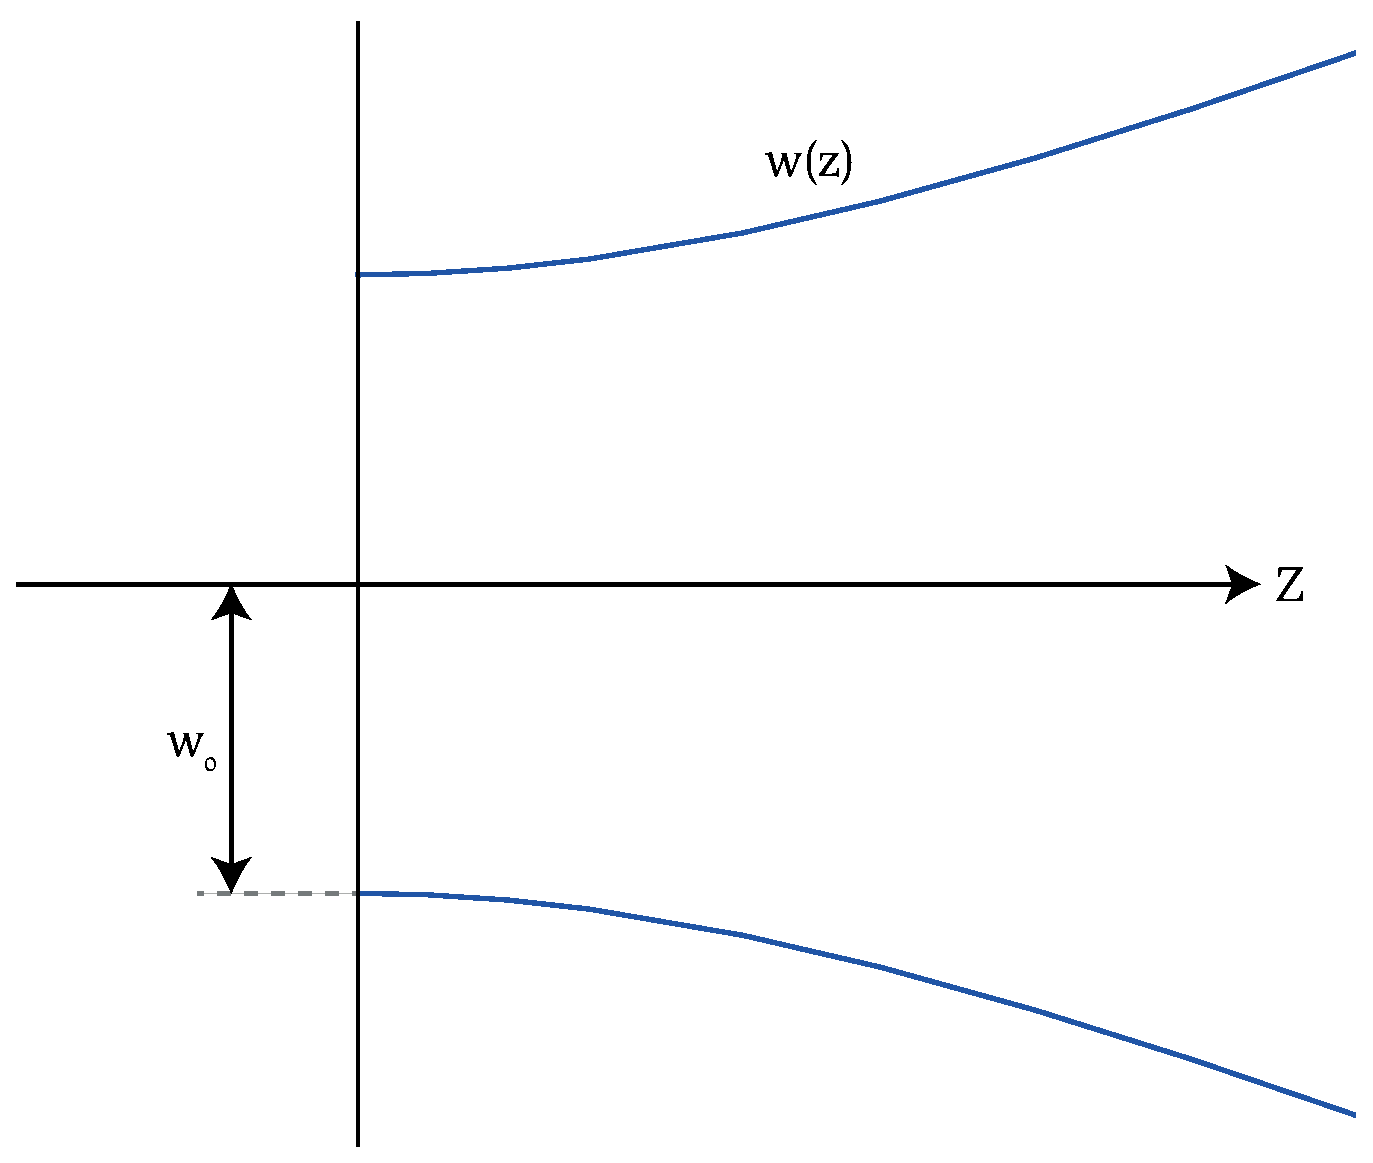
\includegraphics[width=.4\textwidth]{Figures/PropEx.eps}
	\caption{Sketch of Gaussian beam propagation with indication of \(w_0\) and \(w(z)\).}
	\label{PropEx}
\end{wrapfigure}
In our case we want to use a Gaussian microwave. Such beam propagates spatially as shown in \cref{PropEx}.
\(w_0\) is the beam initial beam waist determined by the source and \(w(z)\) is the functino describing the waist. This equation is:
\begin{align}
	w(z) = w_0(z)\sqrt{1+\pqty{\frac{\lambda z}{\pi w_0^2}}^2}\label{wz}
\end{align}
From this equation one can track the spatial propagation of the wave. In this project three sources are given. The initial beam waist is set to \(w_0=\si{0.0275}{\meter}\) corresponding with half a reactor port. With
\begin{align}
	\frac{\lambda z}{\pi w_0^2} = \frac{9.542690316\times10^7 z}{w_0^2 f}
\end{align}
, and \(f\) being the frequency, the sources' beam waists are given as such:
\begin{align}
	\SI{60}{\giga\hertz}  & : \quad w(z)=0.0275\sqrt{\pqty{1+\frac{9.542690316\times10^7 z}{0.0275^2 \ 60\times10^9}}^2}\label{60}   \\
	\SI{98}{\giga\hertz}  & : \quad w(z)=0.0275\sqrt{\pqty{1+\frac{9.542690316\times10^7 z}{0.0275^2 \ 98\times10^9}}^2}\label{98}   \\
	\SI{130}{\giga\hertz} & : \quad w(z)=0.0275\sqrt{\pqty{1+\frac{9.542690316\times10^7 z}{0.0275^2 \ 130\times10^9}}^2}\label{130}
\end{align}
For the three given sources in this project, the beam waist has been plotted on \cref{BeamProp}
\newline

\begin{figure}[H]
	\centering
	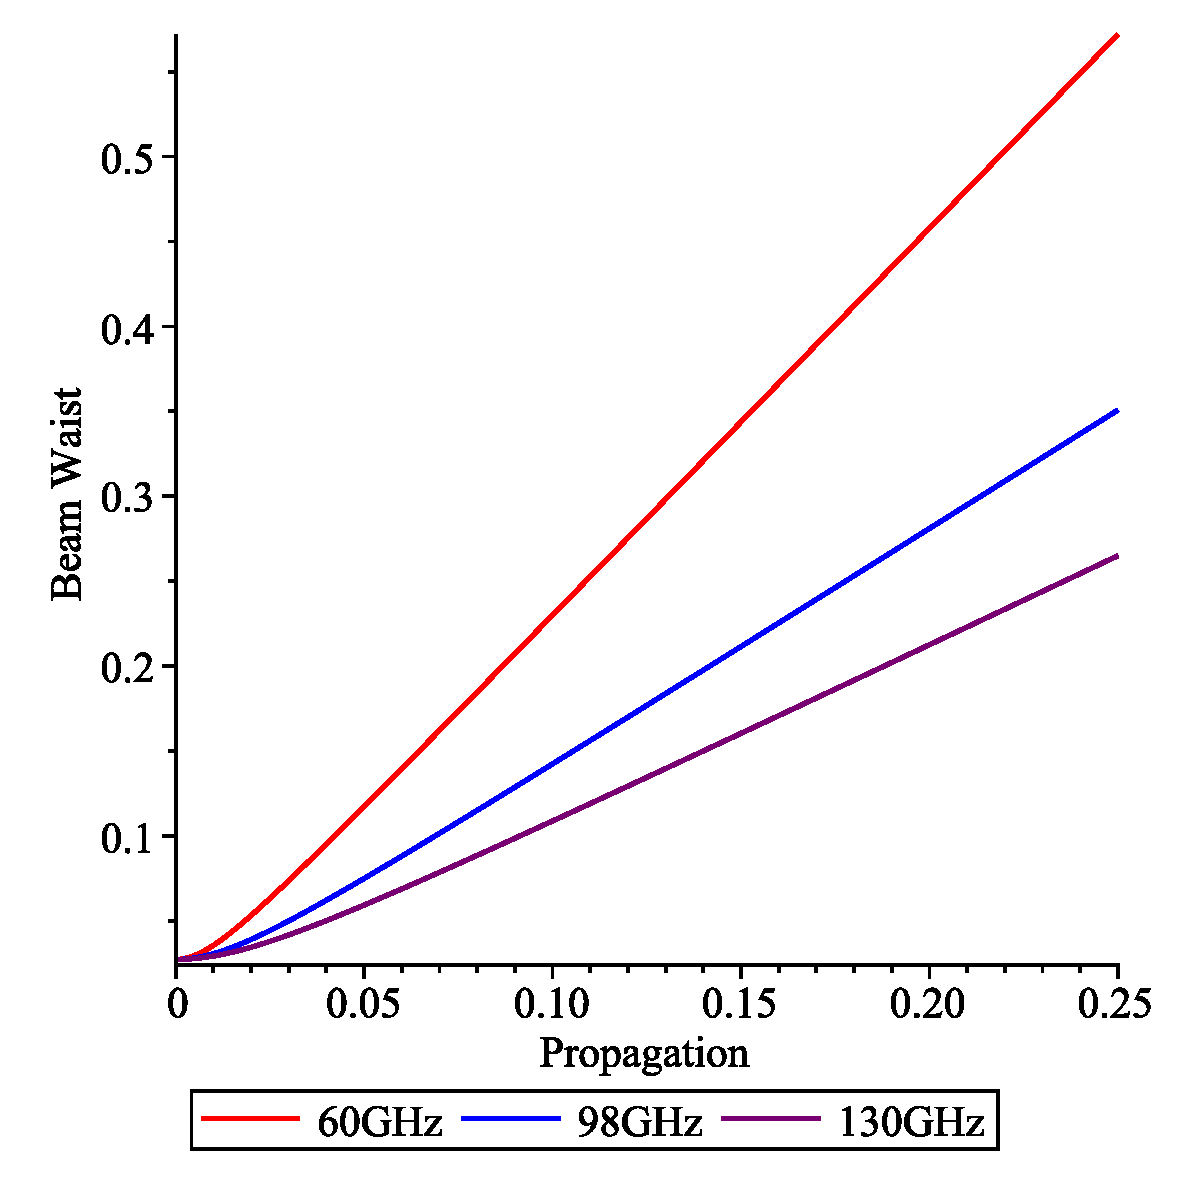
\includegraphics[width=.5\textwidth]{Figures/BeamProp.eps}
	\caption{Beam Waist for the three microwave sources. The functions are \cref{60,98,,130}.}
	\label{BeamProp}
\end{figure}
It is undesireable for some of the beam to not reach the output port and instead propagate into the reactor wall, as this will result in a lesser signal strength. Therefore it can be nesessary to deploy a gaussian telescope.
\subsection{Gaussian beam telescope interferometer}
In order to control the beam waist, one can use a Gaussian beam telescope arrangement around the reactor. A lens is placed between the source and the reactor input port and again between the output port and the reciever. From chapter 5 in ``Fusion Plasma Diagnostics with mm-Waves''\cite{PlasmaDiagnosis} the authors explains how such an arrangement can be obtained. Starting with the focal lengths of the lenses,
\begin{align}
	d = f_0 + f_1
\end{align}
, where \(f_0\) and \(f_1\) are focal lengths, and \(d\) are the distance between the lenses.
The resulting narrowest beam waist after the second lens are given as:
\begin{align}
	w_2 = \frac{f_1}{f_0}w_0
\end{align}
This making the transformation wavelength independent\cite[Eq 5.118]{PlasmaDiagnosis}.
The distance to this waist is given as:
\begin{align}
	d_3 = \frac{f_1}{f_0}\pqty{f_0+f_1-\frac{f_1}{f_0}d_0}
\end{align}
The waist in between the lenses is given as:
\begin{align}
	w_1 = \frac{\lambda f_0}{\pi w_0}
\end{align}
And the distance from the first lens to this waist is:
\begin{align}
	d_1 = \pqty{\frac{\frac{d_0}{f_0}-1}{\frac{w_0^2\pi}{f_0\lambda}+\pqty{\frac{d_0}{f_0}-1}^2}+1}f_0
\end{align}
Thus the distance from \(w_1\) to the second lens is:
\begin{align}
	d_2 = d-d_1
\end{align}
Knowing these variables and utilising \cref{wz} we can model a complete setup. Using the matlab code in \cref{inter}, the following parameters were input:
\begin{align}
	\mqty{r_p = \SI{0.055}{\meter} & r = \SI{0.125}{\meter}  & w_0 = \SI{0.0275}{\meter} & freq = \SI{60}{\giga\hertz}        \\
	d_0 = \SI{0.20}{\meter}        & d_r = \SI{0.10}{\meter} & f_0 = \SI{0.25}{\meter}   & \SI{0.20}{\meter}} \label{interin}
\end{align}
With \(r_p\) being the tokamak port radius, \(r\) the tokamak minor radius and \(d_r\) the distance between the first lens and the reactor wall.
In the case of the Danish Tokamak Undertaking, two ports opposing each other is ideal for use with interferometry. In this example, the port radius, \(r_p\), and the minor radius \(r\) are based on the ST-25 in the basement of building 309 at DTU.
The script gave the results:
\begin{align}
	\mqty{w_1 = \SI{0.0145}{\meter} & w_2 = \SI{0.0220}{\meter}                                            \\
	d_1 = \SI{0.2243}{\meter}       & d_2 = \SI{0.2257}{\meter} & d_3 = \SI{0.232}{\meter}}\label{interou}
\end{align}
Furtermore the code plots a sketch of the desired interferometer setup. The sketch can be seen in \cref{AWESOME}.\newline
\begin{figure}
	\centering
	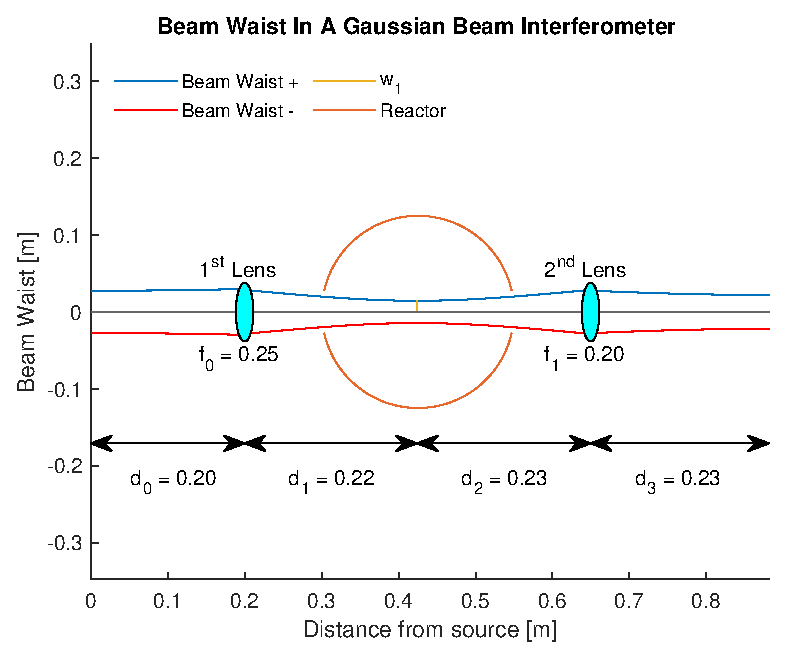
\includegraphics[width=.7\textwidth]{MatlabFigures/Interferometer/Interferometer.eps}
	\caption{Gaussian beam telecsope interferometer setup with input parameters shown in \cref{interin} and output parameters shown in \cref{interou}}
	\label{AWESOME}
\end{figure}
\begin{wrapfigure}[14]{r}{.3\textwidth}
	\centering
	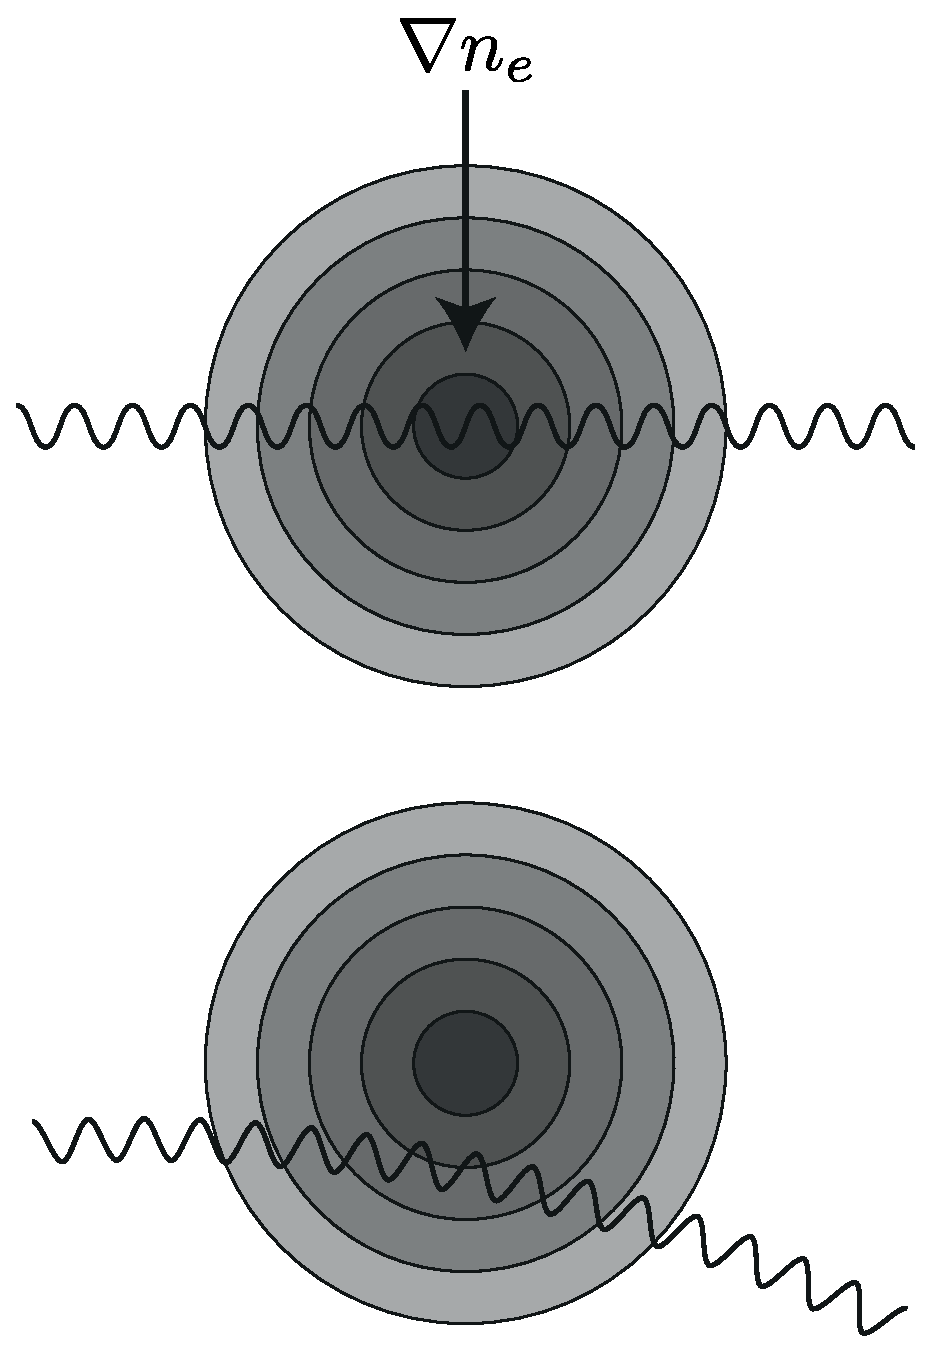
\includegraphics[width=.3\textwidth]{Figures/Refraction.eps}
	\caption{Refraction of the probing beam at center  (top) and off center (bottom).}
	\label{Refrac}
\end{wrapfigure}
Lastly it should be mentioned that the beam waist confinement does not matter if the wave is refracted into the side of the reactor. As the plasma density varies from the center and out, the plasma itself act as a variable lens with variable refractive indices. If the beam is emitted straight through the center, the refractive indices will only shorten and lengthen the wavelength back to normal, however if the beam is emmited off center, it will be refracted away from the center. In such a setup, further calculations need to be conducted to determine variation in signal strength, phase and wavelength. The two described setups are depicted on \cref{Refrac}.
